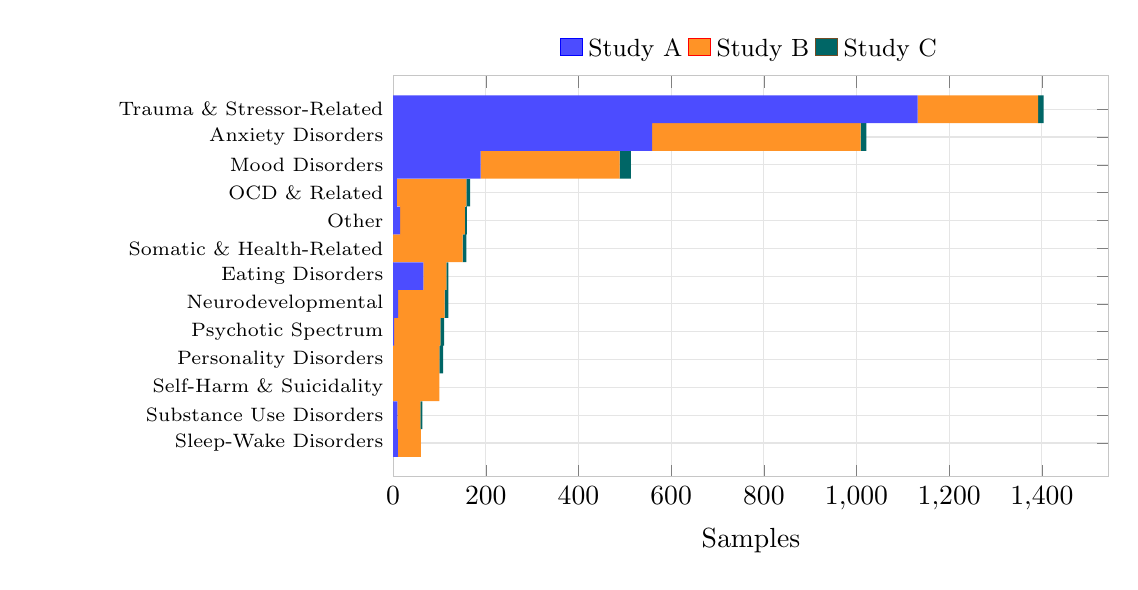
\begin{tikzpicture}
\begin{axis}[
  width=0.88\textwidth,
  height=0.55\textwidth,
  xbar stacked,
  xmin=0,
  ytick=data,
  yticklabels={{Trauma \& Stressor-Related},{Anxiety Disorders},{Mood Disorders},{OCD \& Related},{Other},{Somatic \& Health-Related},{Eating Disorders},{Neurodevelopmental},{Psychotic Spectrum},{Personality Disorders},{Self-Harm \& Suicidality},{Substance Use Disorders},{Sleep-Wake Disorders}},
  y dir=reverse,
  yticklabel style={font=\scriptsize, text width=4.4cm, align=right},
  xlabel={Samples},
  legend style={at={(0.5,1.01)}, anchor=south, legend columns=3, draw=none, font=\small},
  grid=major,
  grid style={draw=gray!20},
  axis line style={draw=gray!45},
]
\addplot+[draw=none, fill=blue!70] coordinates {(1132,0) (559,1) (189,2) (8,3) (15,4) (0,5) (65,6) (11,7) (2,8) (0,9) (0,10) (9,11) (10,12)};
\addlegendentry{Study A}
\addplot+[draw=none, fill=orange!85] coordinates {(260,0) (450,1) (300,2) (150,3) (140,4) (150,5) (50,6) (100,7) (100,8) (100,9) (100,10) (50,11) (50,12)};
\addlegendentry{Study B}
\addplot+[draw=none, fill=teal!80!black] coordinates {(12,0) (12,1) (24,2) (8,3) (4,4) (8,5) (4,6) (8,7) (8,8) (8,9) (0,10) (4,11) (0,12)};
\addlegendentry{Study C}
\end{axis}
\end{tikzpicture}
